% !TeX program = xelatex
\documentclass[11pt,a4paper]{article}
\usepackage[margin=24mm]{geometry}
\usepackage{amsmath,amssymb,booktabs,array,tikz}
\usetikzlibrary{arrows.meta,positioning}
\usepackage[hidelinks]{hyperref}
\title{Prior-Art Comparison: Findings and Research Decision}
\author{Internal assessment}
\date{November 21, 2026}
\begin{document}\maketitle
\noindent\textbf{Conclusion.} The central idea of constructing an untimed,
collision-free completion schedule from partial-path sweep conflicts and
movement/wait commands is established prior art. Our finite point-duplication
model can be reduced to the classical segment-progress model described below.
The sixteen endpoint classes remain a useful restricted corollary, but no
independent novelty claim is established. This assessment does not claim an
exhaustive historical search or proof that no publishable extension exists.

\section{The most direct predecessor is from 1989}
O'Donnell and Lozano-P\'erez [1] are a closer conceptual predecessor than SCALE
for our basic construction problem. Their task-completion diagram uses two
axes of ordered path segments. A cell records whether the two segment sweeps
intersect. Safe schedules move horizontally, vertically, or diagonally through
the diagram; these correspond to one robot moving, the other moving, or both.
They construct schedules and discuss asynchronous START/WAIT execution.

Two details are particularly important. Printed page 486 adds null endpoint
segments and handles blocking by final parked robots (Figure 3). Printed page
487 describes global schedule search even when purely sequential whole-path
execution is unsafe. Thus endpoint persistence and partial-progress solutions
must not be described as absent from the classical literature.

\begin{center}\small
\begin{tabular}{p{48mm}p{91mm}}\toprule
Our terminology & Corresponding classical construction\\\midrule
Partial-path sweep & Swept volume associated with a path segment.\\
Point sweep / waiting footprint & Null segment representing an endpoint position.\\
Sweep-pair compatibility & Unshaded segment-pair cell / compatible swept volumes.\\
Tuple execution stage & A permitted joint segment-progress step.\\
Wait duplication & Leave one progress coordinate unchanged while advancing another.\\
Untimed precedence execution & Ordered START/WAIT commands, triggered by segment completion.\\\bottomrule
\end{tabular}
\end{center}
This is a correspondence of model operations, not a claim that our Python code
is a port of the authors' implementation. The original application is robot
manipulators; their occupancy predicates use conservative geometric models.
The diagram's rectangular cells are pairs of path segments, not a partition
of the physical workspace into grid cells.

\clearpage
\section{An explicit reduction of our two-robot finite model}
Let $P_i=(p_{i,0},\ldots,p_{i,m})$ and
$P_j=(p_{j,0},\ldots,p_{j,n})$. Hold paths, permissible vertex stops,
footprints, and sweep predicates fixed. Define
\begin{equation}
Q=\{0,\ldots,m\}\times\{0,\ldots,n\}.
\end{equation}
A state $(k,l)$ places the centers at $p_{i,k}$ and $p_{j,l}$.
Choose $(d_i,d_j)$ from $(1,0)$, $(0,1)$ or $(1,1)$, within the path bounds.
The transition to $(k+d_i,l+d_j)$ is allowed exactly when
\begin{equation}
S_i[k,k+d_i]\cap S_j[l,l+d_j]=\varnothing.\label{eq:step}
\end{equation}
An unchanged coordinate uses a point sweep, including at a final destination.
Initial configurations must also have disjoint footprints. This is the
segment/move/wait abstraction obtained from the classical diagram with explicit
endpoint occupancy, expressed using our notation. We do not identify it with
unrestricted continuous configuration-space planning.

\begin{center}
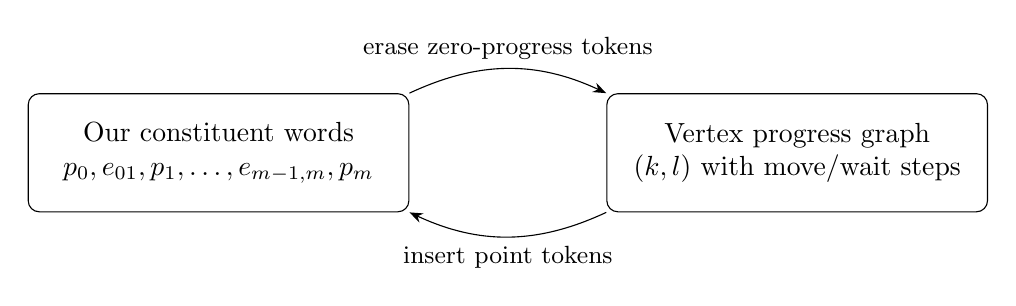
\begin{tikzpicture}[>=Stealth,node distance=10mm,
box/.style={draw,rounded corners,align=center,text width=46mm,minimum height=15mm}]
\node[box] (word) {Our constituent words\\$p_0,e_{01},p_1,\ldots,e_{m-1,m},p_m$};
\node[box,right=25mm of word] (progress) {Vertex progress graph\\$(k,l)$ with move/wait steps};
\draw[->] (word.north east) to[bend left=25] node[above,font=\small] {erase zero-progress tokens} (progress.north west);
\draw[->] (progress.south west) to[bend left=25] node[below,font=\small] {insert point tokens} (word.south east);
\end{tikzpicture}
\end{center}

\textbf{Proposition (reachability equivalence for the fixed finite model).}
Our exhaustive point-duplication solver has a completion witness if and only if
the graph in Equation~\eqref{eq:step} has a path from $(0,0)$ to $(m,n)$.

\textbf{Forward direction.} Read a solver witness in order. A consumed point
constituent does not change the physical vertex. A consumed edge advances its
vertex by one. Treat point consumption as waiting and delete stages with no
physical advancement. Every remaining stage satisfies Equation~\eqref{eq:step}
because it has the same physical sweeps as the original stage. Endpoints persist.

\textbf{Reverse direction.} Before a progress step, consume any pending original
point tokens at the current safe positions, while the other robot waits there.
Then consume the edge tokens for that step, using point waiting for unchanged
coordinates. At the resulting safe configuration, consume the newly pending
point tokens as needed. Repeat and consume final point tokens. Each inserted
point-only stage is safe because its footprints are subsets of a safe adjoining
stage, or belong to the safe initial configuration. No non-point token is copied
and original token order is preserved. The finite graph path therefore expands
to a finite solver witness. $\square$

This reduction shows why extra point tokens change bookkeeping and stage counts
without creating a new two-robot reachability principle. Stage-count optima and
physical makespan need not be preserved by the reduction.

\clearpage
\section{Checked example and the role of the endpoint table}
For the existing five-edge-per-robot example
\begin{center}\small\texttt{02\_10\_RobotPath\_AlternatingProgress}\end{center}
the adapted progress graph has
$6\times6=36$ possible states, 32 reachable states and 73 accepted directed
transitions. A completion path is
\begin{equation}
(0,0)\to(1,1)\to(2,2)\to(3,3)\to(4,4)\to(5,5).
\end{equation}
Its edges use full-sweep disjointness, so no exact simultaneous timing within
a stage is required. The earlier three-block alternating witness is another
valid plan, not the only possible one. This check adapts the published model
using our geometry; it does not run the 1989 authors' software.

\subsection*{Where our sixteen classes sit}
The general endpoint formula is
\begin{equation}
F_{ij}=(\neg\sigma_{j|i}\land\neg\varepsilon_{i|j})
\lor(\neg\sigma_{i|j}\land\neg\varepsilon_{j|i}).
\end{equation}
Here $\sigma_{j|i}$ tests whether $j$'s initial footprint intersects $i$'s full
sweep; $\varepsilon_{i|j}$ tests whether $i$'s final footprint intersects $j$'s.
The other two flags exchange roles. For arbitrary paths this certifies a
whole-route serial schedule, not all possible schedules.

In the restricted grid/common-centerline-arc domain of our proof audit,
endpoint membership equals this geometric test and the three obstruction types
make $F_{ij}$ necessary as well as sufficient. Consequently this restricted
predicate decides whether the adapted classical progress graph has a completion
path, without searching all of it. This is \emph{our derivation of the
correspondence}, not an attributed theorem quoted from a predecessor.

\textbf{Historical finding.} In the texts inspected, we did not locate the
identical four-bit table or its exact restricted proposition stated verbatim.
That negative search result does not prove novelty. The existing literature
already constructs schedules for a broader segment-conflict input, including
endpoint blocking. A simple special-case characterization needs its own
novelty and significance justification; a change of notation is insufficient.

\section{Acyclic priorities: a theorem with a directly comparable proof}
Gr\'egoire et al. [2, Sec.~3.2, Theorem 3; PDF p.~11] prove feasibility of
acyclic priority graphs by topologically ordering the robots and letting each
complete while the others wait. This is the same constructive proof pattern as
our acyclic serialization certificate. Their Sec.~2.1 assumes convex pairwise
collision cross-sections and safe boundary positions. They therefore do not
directly provide our endpoint-interference table; we must not transplant their
conclusion to our different endpoint assumptions without checking them.

Leroy et al. [3, Secs.~3--4] use bounding-box coordination diagrams and a
resolution-complete search construction for their specified model. Their
discussion allows backward progress. This distinguishes their feasible-motion
set from our forward-only one; it does not make our finite search a new concept.

\clearpage
\section{Decision on the present claims}
\begin{center}\small
\begin{tabular}{p{60mm}p{80mm}}\toprule
Proposed claim & Assessment after the comparison\\\midrule
First sweep-based fixed-path collision-free execution framework & Unsupported:
the central segment-sweep/START-WAIT construction is explicit in 1989.\\
New feasibility principle from point-sweep duplication & Unsupported by the
current operation alone: the finite reachability models reduce to one another.\\
New general completion guarantee from acyclic priorities & Not justified:
the same proof pattern has an explicit predecessor, with assumptions to compare.\\
New universal sixteen-case feasibility test & Incorrect scope: equivalence
was argued only for a restricted common-centerline-arc model.\\
Useful explicit endpoint classification & Supported within its stated domain;
novelty and publication-level significance remain unestablished.\\
Validated RMFS execution implementation & A concrete engineering result;
not by itself a new theoretical framework or a performance advantage.\\\bottomrule
\end{tabular}
\end{center}

\paragraph{Research decision.}
Do not expand the present manuscript as a new general theory of sweep management
on the strength of the currently audited results. Keep its implementation,
examples and proofs as a reproducible foundation. The evidence supports
rediscovery and a useful specialized formulation, not a demonstrated new
general solution. This is an assessment of the current claims, not a conclusion
that the project must be abandoned.

\paragraph{What the next research must add.}
Before another large experiment, select a precise result not supplied by the
above correspondence: for example, a demonstrably useful stronger geometric
feasibility shortcut, or a route-generation method evaluated against applicable
planning baselines. Merely adding simulation-based evaluation, a different
objective, or more robots does not establish novelty. PathPlanner architecture
and new control objects require a separate design discussion; none was added.

\paragraph{Completed work and limits.}
The 1989 scanned paper was inspected visually, particularly printed pp.~485--489.
The 2015 paper's formal assumptions and Theorem 3 proof were read directly;
the 1999 paper's construction and completeness discussion were checked. The
comparison includes an explicit finite-model reduction and a concrete graph
check, rather than a speed guess based on MILP. It is not a historical priority
proof, an independent reproduction of the external software, or a theorem
covering arbitrary continuous timed executions. The main research paper,
Korean documents and production code remain unchanged.

\begin{thebibliography}{9}\small
\bibitem{odonnell} P. A. O'Donnell and T. Lozano-P\'erez, ``Deadlock-Free and
Collision-Free Coordination of Two Robot Manipulators,'' ICRA, 484--489, 1989.
\url{https://lis.csail.mit.edu/pubs/tlp/coordination-o-donnell.pdf}.
\bibitem{gregoire} J. Gr\'egoire, S. Bonnabel, and A. de La Fortelle,
``Robust multirobot coordination using priority encoded homotopic constraints,''
arXiv:1306.0785v3, 2015, Secs.~2.1 and 3.2.
\url{https://arxiv.org/html/1306.0785v3}.
\bibitem{leroy} S. Leroy, J.-P. Laumond, and T. Sim\'eon, ``Multiple Path
Coordination for Mobile Robots: A Geometric Algorithm,'' IJCAI, 1118--1122,
1999. \url{https://ijcai.org/proceedings/1999/159}.
\end{thebibliography}
\end{document}
